\section{Vergleichbare Arbeiten und Projekte}
\label{sec:related-work}

Andere Entwicklungsumgebungen für Datenbanken und auch Generatoren für Abfragemasken gibt es in schier unüberblickbarer Zahl. Dieses Kapitel stellt einige der vefügbaren Programme oder Bücher und hebt dabei insbesondere den Einfluss hervor, den sie auf esqulino direkt oder indirekt genommen haben. Sinn dieses Kapitels ist damit der "`Blick über den Tellerrand"' um aus der Vielzahl an verfügbaren Ideen jene herauszustellen die für diese Arbeit von Bedeutung sind. Es handelt sich nicht um eine strukturierte Bewertung oder Einordnung dieser Inspirationsquellen.

\subsection{Software: Scratch}

\begin{figure}[p]
  \centering 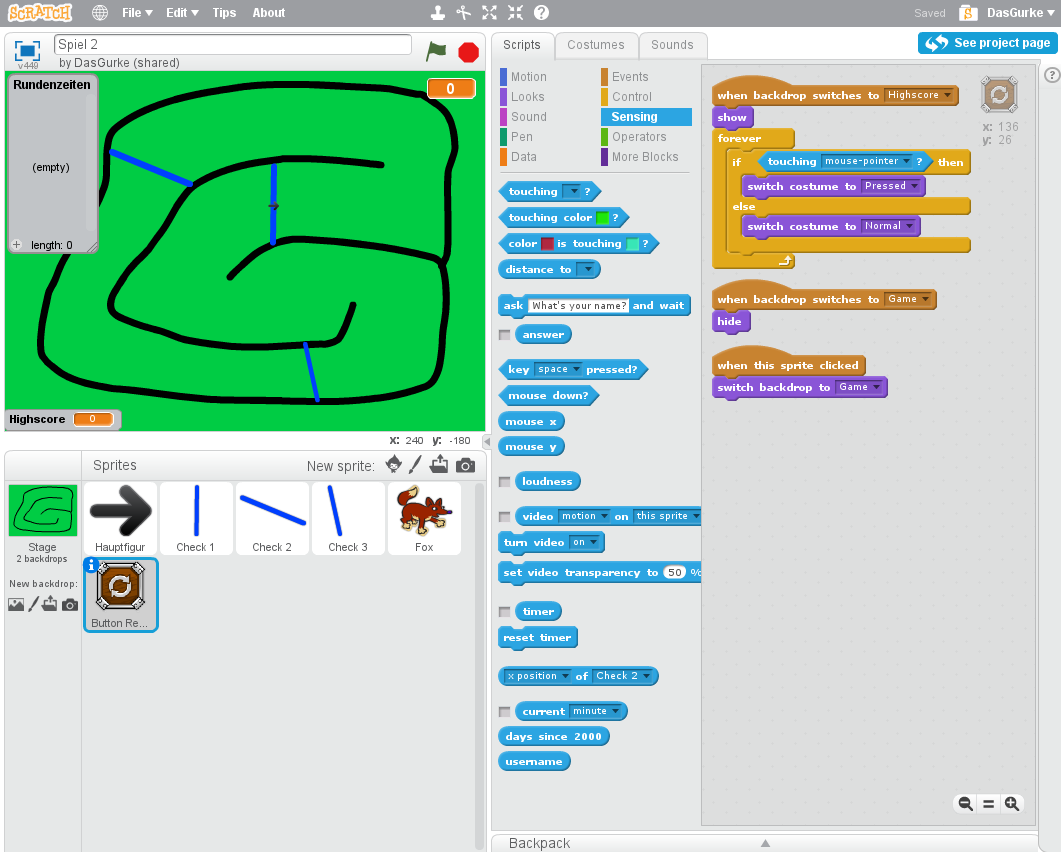
\includegraphics[width=0.7\textwidth]{images/related-work-scratch-editor-full.png}
  \caption{Der Scratch-Editor mit einem Beispielprojekt aus Sicht eines Entwicklers}
  \label{fig:scratch-editor-full}
\end{figure}

\begin{figure}[p]
  \centering 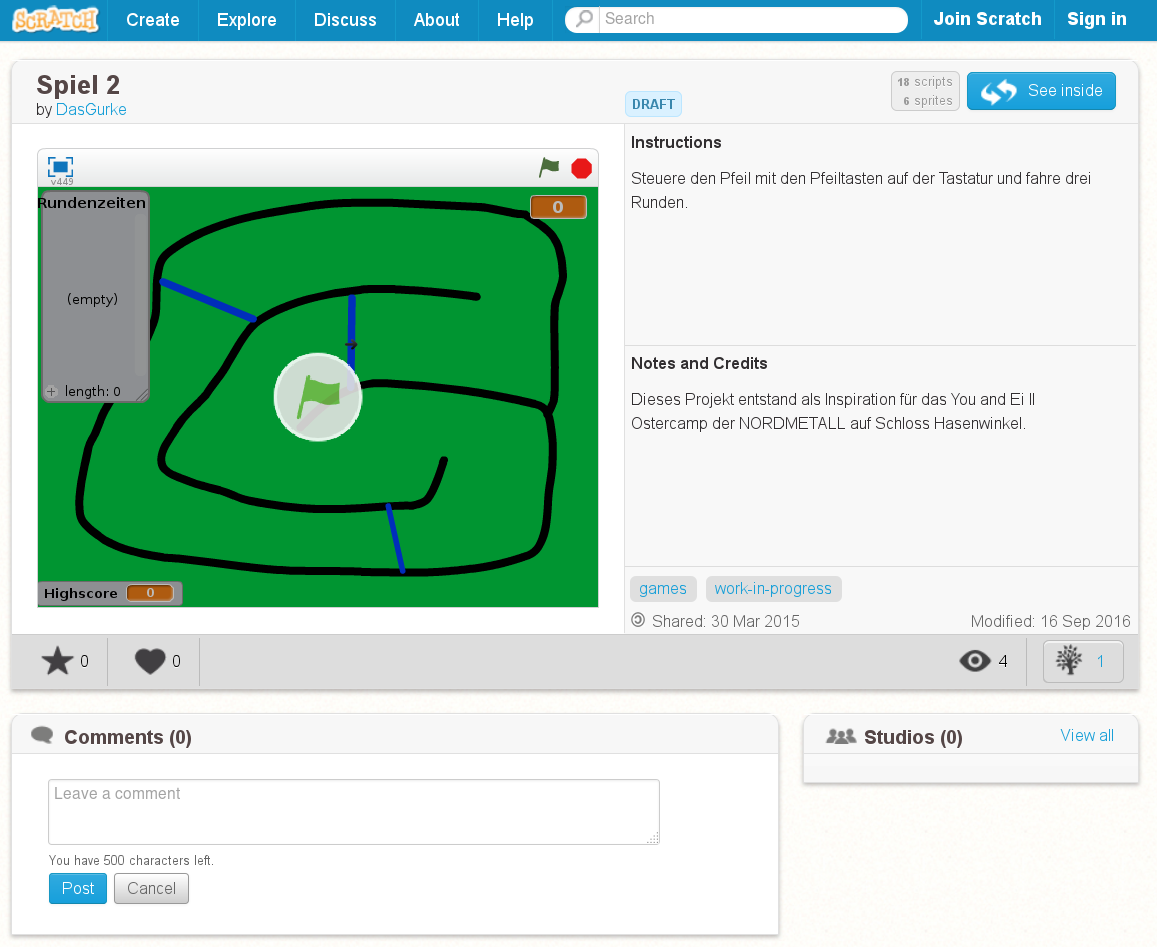
\includegraphics[width=0.7\textwidth]{images/related-work-scratch-project-full.png}
  \caption{Ein Scratch Projekt mit kurzen Handlungsanweisungen und einem Kommentarbereich in der Sicht für Endanwender.}
  \label{fig:scratch-enduser-full}
\end{figure}


Diese Masterarbeit zieht eine Menge Inspiration aus dem Scratch-Project des Massachusetts Institute of Technology (MIT)\footnote{\url{https://scratch.mit.edu/}}. Bei Scratch handelt es sich um eine Entwicklungsumgebung speziell für Kinder und Jugendliche deren bestimmendes Bedienkonzept Drag \& Drop ist. Scratch lehrt den Umgang mit imperativen und ereignisorientierten Programmierkonzepten und ist damit in Bezug auf die zu vermittelnden Inhalte von dieser Thesis doch deutlich entfernt. Abbildung \ref{fig:scratch-editor-full} zeigt wie die Oberfläche von Scratch für einen Entwickler aussieht, Abbildung \ref{fig:scratch-enduser-full} demonstriert wie sich ein Projekt initial einem Endanwender präsentiert.

Im weiteren Verlauf der Arbeit wird jedoch noch deutlich werden, dass sich esqulino an vielen Stellen dennoch sehr stark an Scratch orientiert. So nutzt auch esqulino einen Drag \& Drop Editor um Syntaxfehler von vornerein auszuschließen und kontextsensitiv mögliche Operationen hervorzuheben. Die Verwendung eines, zu diesem Zeitpunkt allerdings nicht vollständig ausgearbeiteten, Farbkonzeptes nimmt sich ebenfalls Scratch zum Vorbild. Und schließlich ist auch die Zweiteilung eines Projekts in eine Besucheransicht sowie eine Entwickleransicht sowie der fließende Wechsel zwischen diesen Modi eine direkte Inspiration.

Scratch baut dabei nicht auf einer bestehenden Programmiersprache auf, sondern nutzt eine eigene Sprache. Die Schlüsselwörter dieser Sprache, wie auch die Oberfläche des Editors, sind dabei in viele verschiedene natürliche Sprachen (Englisch, Deutsch, Spanisch, ...) übersetzt worden. Esqulino geht an dieser Stelle einen anderen Weg und lehrt unmittelbar den Umgang mit SQL und HTML, allerdings in gegebenenfalls redizierten Umfängen (siehe \ref{sec:sql-subset} \nameref{sec:sql-subset} und \ref{sec:design-ui-concept} \nameref{sec:design-ui-concept}).

Letztendlich liegen die Wurzeln dieser Arbeit definitiv bei Scratch: Der Arbeitstitel lautete "`Scratch für SQL und Webanwendungen"' und weckt bei Leuten, die mit Scratch schon vertraut sind, auch die richtigen Assoziationen.

\subsection{Software \& Kurs: SqlZoo}

\begin{figure}[p]
  \centering \includegraphics[width=\textwidth]{images/related-work-sql-zoo.png}
  \caption{Ergebnisansicht mit aktiviertem Hinweis für eine einzelne Aufgabe des SqlZoo.}
  \label{fig:sqlzoo-check-result}
\end{figure}

\begin{figure}[p]
  \centering \includegraphics[width=\textwidth]{images/related-work-sql-zoo-error.png}
  \caption{Technische Fehlermeldung einer Datenbank aufgrund eines Syntaxfehlers in der Eingabemaske von SqlZoo.}
  \label{fig:sqlzoo-check-result}
\end{figure}

Bei der Webseite "`SqlZoo"' handelt es sich um eines der wenigen Angebote, die SQL-Kenntnisse vermitteln und sich dabei explizit auch an Kinder wenden. Es handelt sich dabei sowohl um einen Kurs in Form einer Sammlung von aufeinander aufbauenden Aufgaben inklusive begleitendem Lehrmaterial als auch eine vergleichsweise rudimentäre, webbasierte Software in welcher die Lernenden ihre ersten Schritte mit SQL machen. Anders als in Scratch erfolgt die Programmierung der nötigen Abfragen in einem normalen Textfeld, auch Syntax-Hervorhebung ist nicht vorhanden.

Inhaltlich präsentiert sich das Projekt als eine Sammlung von Aufgaben. Diese sind thematisch in Kapitel untergliedert und nutzen in der Regel einen sehr überschaubaren Datenbestand. Die Ergebnisse werden neben dem Textfeld angezeigt und mit dem korrekten Ergebnis verglichen (Abbildung \ref{fig:sqlzoo-check-result}. So können Lernende ihre Ergebnisse selbständig kontrollieren, darüber hinaus ist es ebenfalls möglich sich die korrekte Ergebnismenge anzeigen zu lassen und als Lösungshinweis zu nutzen.

Nach den Lerneinheiten folgt dann eine Serie von Quizfragen bei denen unter anderem zu einer Ergebnismenge die zugrundeliegende Abfrage gewählt werden muss. Die Invertierung dazu wird ebenfalls abgefragt: Es wird eine Abfrage gezeigt und es muss die korrekte Ergebnismenge gewählt werden. Weitere Aufgabentypen beschäftigen sich zum Beispiel mit der Wahl der korrekten SQL-Formalisierung zu einer natürlichsprachlich formulierten Anfrage.

Ein Alleinstellungsmerkmal dieses Angebots ist die sehr breite Unterstützung verschiedener Datenbanksysteme. Als Lernender kann man die Aufgaben wahlweise mit dem Microsoft SQL Server, Oracle, MySQL, DB2, Ingres oder PostgreSQL lösen. SqlZoo wir ebenfalls in mehreren Sprachen angeboten, die deutsche Übersetzung ist allerdings nicht durchgehend verfügbar.

Es ist mit dem SqlZoo prinzipiell auch möglich mutierende Abfragen auszuführen. Diese werden allem Anschein nach allerdings nicht über eine einmalige Anzeige hinaus persistiert. Da die Seite auch keinen Login vorsieht, wäre es aber auch prinzipiell nur schwer vorstellbar Persistenz über mehrere Browsersitzungen hinweg herzustellen. Alle mutierenden Operationen, es wird zum Beispiel auch \lstinline{CREATE TABLE} behandelt, sind dabei lediglich als Referenz verfügbar und nicht Teil des Kurses.

\subsection{Software: App Inventor}

Bei dem AppInventor handelt es sich um eine Kollaboration des MIT mit Google und gewissermaßen um eine logische Fortführung von Scratch. Erstellt werden mit dem AppInventor nicht mehr in Webseiten einbettbare Flash-Anwendungen, sondern Apps für das Android Betriebssystem. Wie schon Scratch läuft auch diese Anwendung in einem Webbrowser. Grundsätzlich ist auch diese Webseite in verschiedenen Sprachen verfügbar, Deutsch zählt zum gegenwärtigen Zeitpunkt allerdings nicht dazu.

Im Vergleich zu Scratch ist der AppInventor wesentlich anspruchsvoller, die Struktur der relativ komplizierten Android-Oberflächen wird vor dem Benutzer nicht versteckt, dafür aber in einen WYSIWYG\footnote{"`What You See Is What You Get"' bezeichnet die visuelle Vorschau in einem Editor ohne den Umweg über einen Kompilierungsschritt.}-Editor verpackt. Der zu schreibende Programmcode wird wieder in einer abstrakten Sprache mit Drag \& Drop Elementen formuliert. Daraus wird dann Java-Code erzeugt, diesen bekommt der Entwickler im Normalfall aber nicht zu Gesicht.

Um die Anwendungen zu testen müssen diese auf das Handy der Entwickler geladen oder in einem Emulator ausgeführt werden. Es ist dafür nötig, ein (reales oder emuliertes) Gerät über die "`App Inventor Companion App"' direkt mit der Webseite zu verbinden. Sobald diese Verbindung steht werden die im Browser vorgenommenen Änderungen fast sofort auf dem Smartphone widergespiegelt.

Wie Scratch befördert auch der App Inventor den Austausch von Entwicklern untereinander. Es ist möglich die eigenen Apps in einer Gallerie auszustellen und dort zu den Entwicklungen von anderen Menschen Rückmeldung zu geben.

\begin{figure}[p]
  \centering 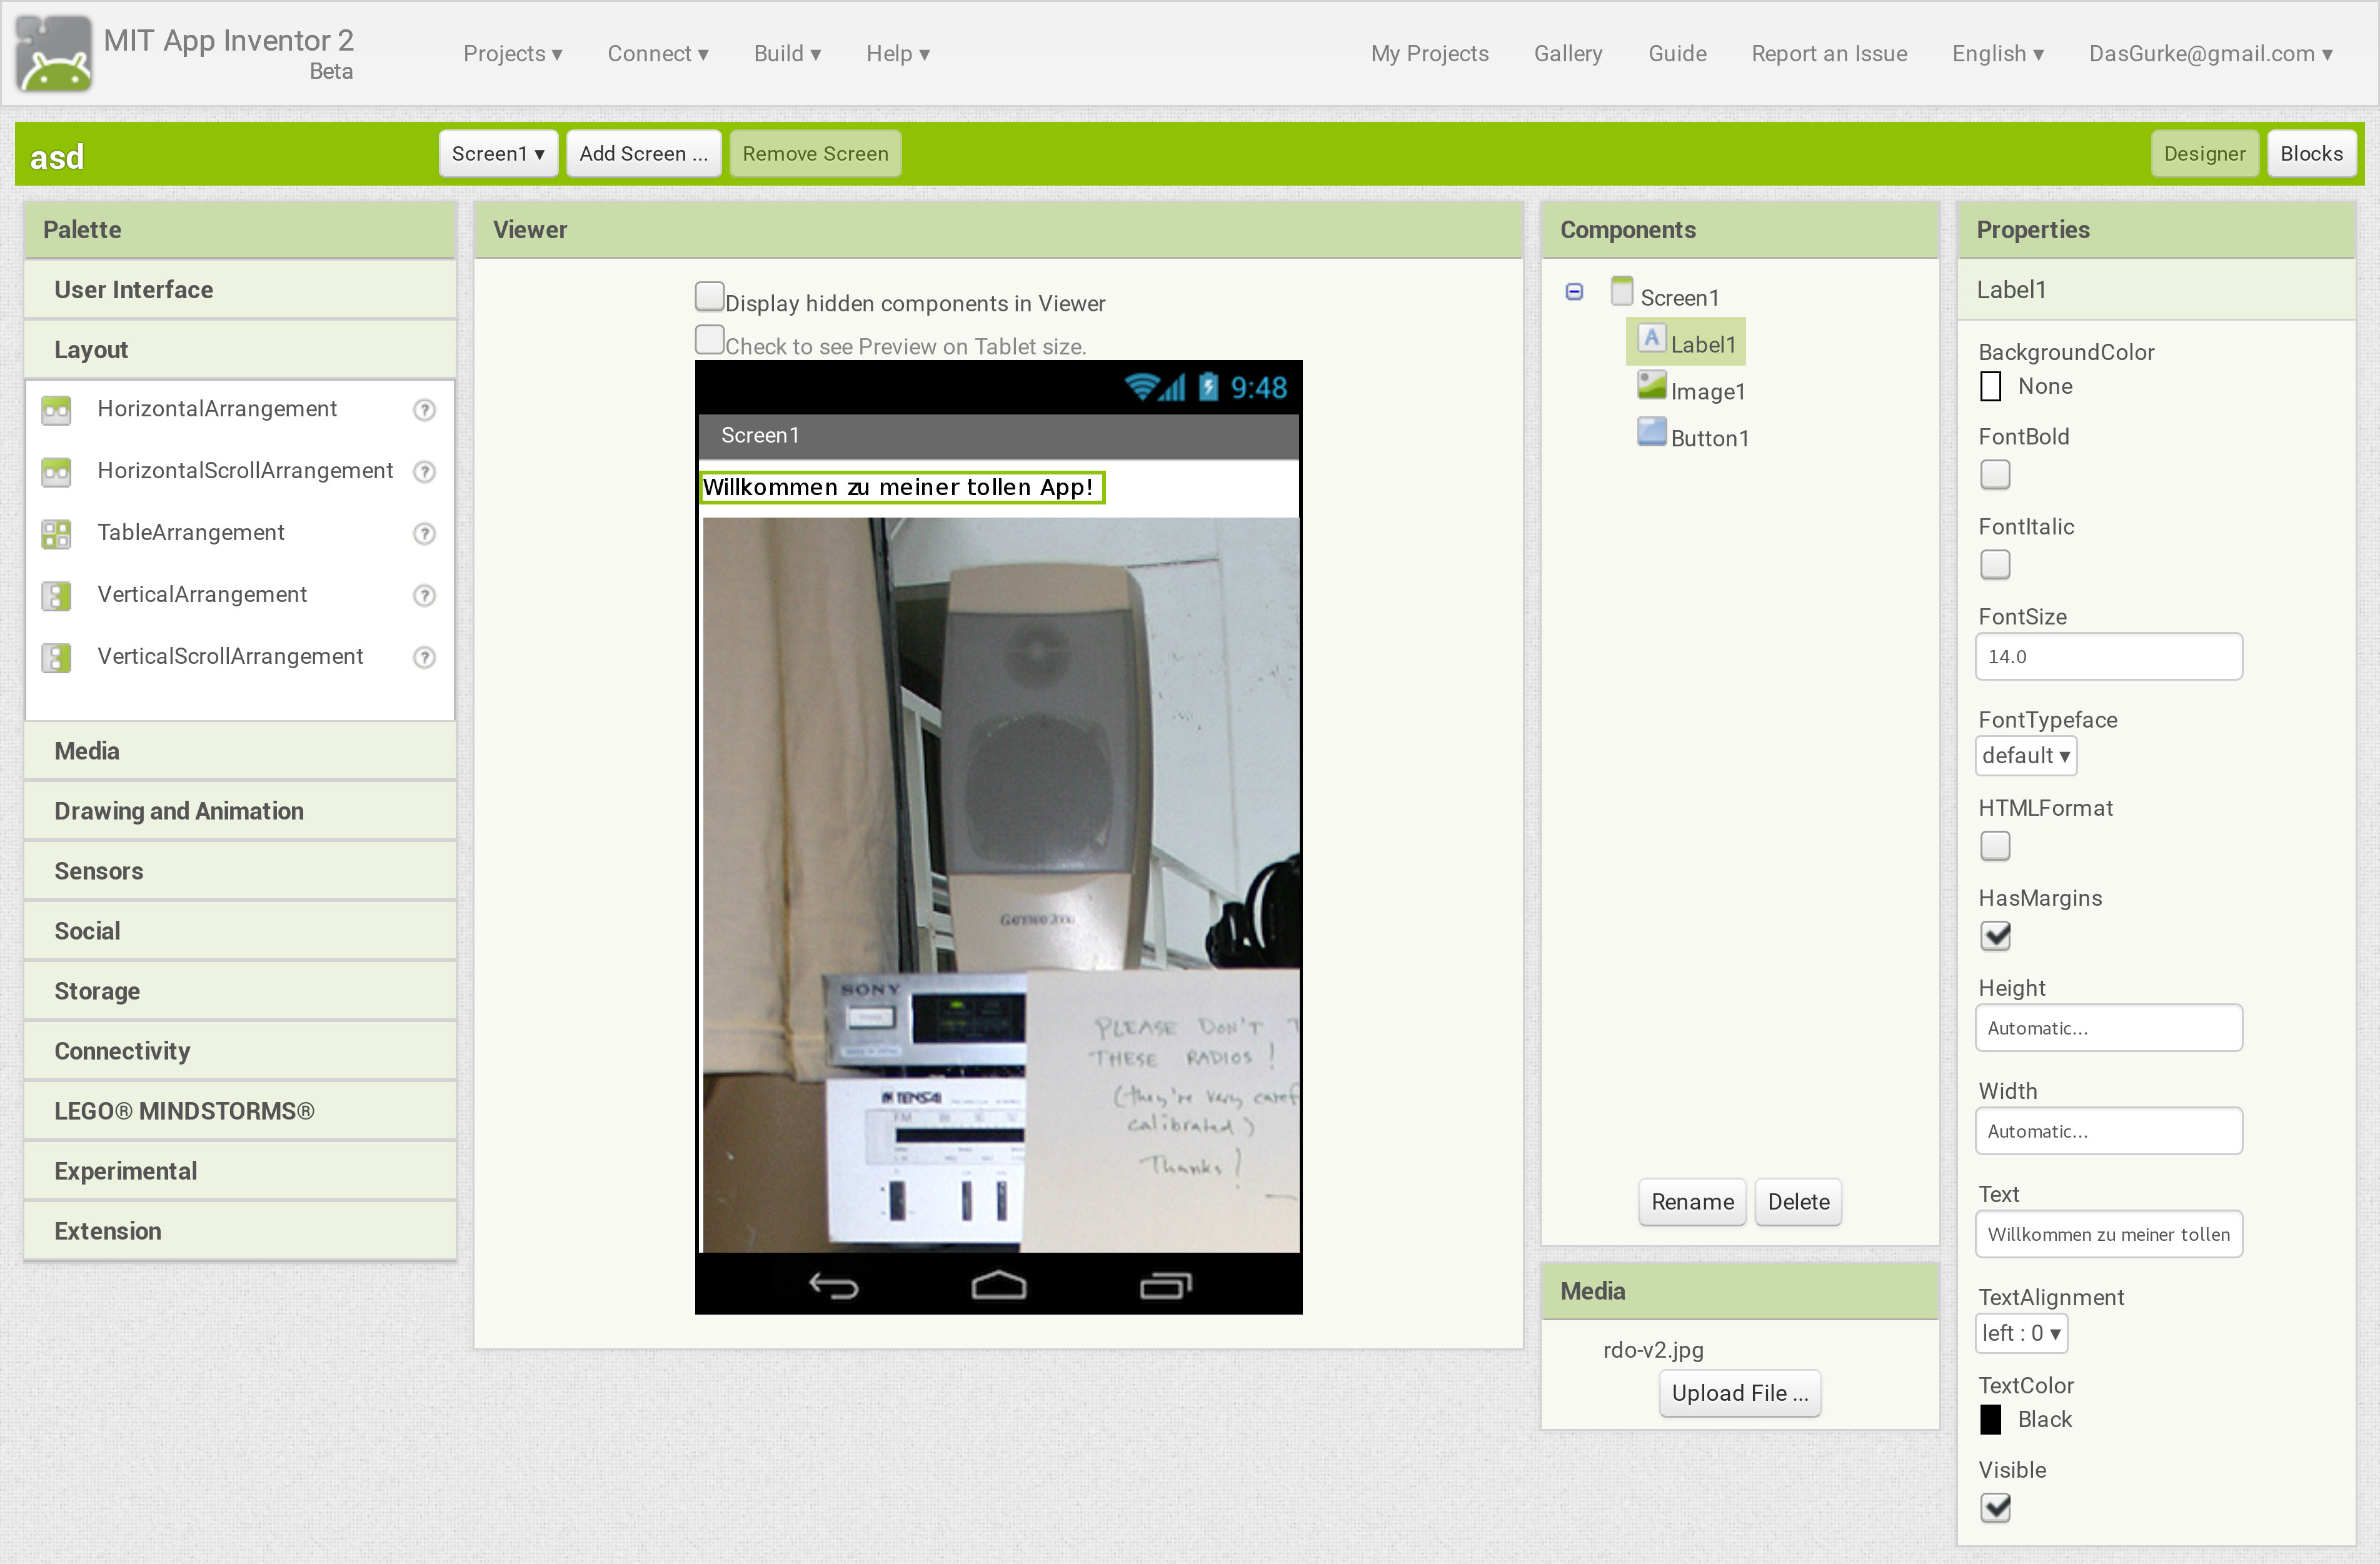
\includegraphics[width=\textwidth]{images/related-work-app-inventor-designer.png}
  \caption{Oberflächeneditor des App Inventor}
  \label{fig:app-inventor-ui-designer}
\end{figure}

\begin{figure}[p]
  \centering \includegraphics[width=\textwidth]{images/related-work-app-inventor-blocks.png}
  \caption{Codeeditor des App Inventor.}
  \label{fig:app-inventor-block-designer}
\end{figure}

\subsection{Software \& Kurs: AppCamps}

\info[inline]{Hamburger Start-Up, dass sich mit einer ebenfalls an Scratch orienterten Entwicklungsumgebung Apps für Smartphones entwickeln können.}


\subsection{Software: Visual Studio Lightswitch}

\info[inline]{Generator für Datengetriebene Geschäftsanwendung mit überschaubarer Applikationslogik.}

\subsection{Buch: Die Macht der Abstraktion}

\info[inline]{Buch zum Einstieg in die Programmierung mit einem interessanten, sehr Datentypgetriebenen Ansatz.}

\info[inline]{Die Dr. Scheme Umgebung und auch die verwendete Sprache heißt jetzt ``Racket'' und wird immer noch weiter entwickelt.}

\subsection{Software: Microsoft Access}

\info[inline]{Eher eine Datenbank als eine sinnvolle Eingabemaske für unversierte Benutzer.}

\subsection{Software: MySQL Workbench}

\info[inline]{Wirklich ein Datenbanktool, keinerlei Benutzerschnittstelle für ``normale'' Benutzer.}

%%% Local Variables:
%%% mode: latex
%%% TeX-master: "thesis"
%%% End:
